\documentclass[12pt,a4paper,final]{article}
\usepackage[left=2.5cm,right=2.5cm,top=2.5cm,bottom=2.5cm]{geometry}

%% IDIOMA
\usepackage[utf8]{inputenc}
\usepackage[portuguese]{babel}

%% TRANSFORMAÇÕES ESTILO CSS
\usepackage{graphicx}

%% ESTÉTICA
\usepackage{enumerate}
\usepackage{booktabs}
\usepackage{amsmath, amsthm, amssymb, amsfonts}
\usepackage{multirow}
\usepackage[hyphens]{url}
\usepackage{subfig}

%% FONTE
\usepackage[T1]{fontenc}
%\usepackage[sc]{mathpazo} % Palatino with smallcaps
\usepackage{mathptmx}
\usepackage{eulervm} % Euler math

%% TIPOGRAFIA
\usepackage{parskip}
\usepackage[activate={true,nocompatibility},final,tracking=true,kerning=true,spacing=true,factor=1100,stretch=10,shrink=10]{microtype}

%% CODIGO
\usepackage{listings}
\usepackage{color}

\definecolor{dkgreen}{rgb}{0,0.6,0}
\definecolor{gray}{rgb}{0.5,0.5,0.5}
\definecolor{mauve}{rgb}{0.58,0,0.82}

\lstset{frame=tb,
  aboveskip=3mm,
  belowskip=3mm,
  showstringspaces=false,
  columns=flexible,
  basicstyle={\small\ttfamily},
  numbers=none,
  numberstyle=\tiny\color{gray},
  keywordstyle=\color{blue},
  commentstyle=\color{dkgreen},
  stringstyle=\color{mauve},
  breaklines=true,
  breakatwhitespace=true,
  tabsize=3
}

\title{Relatório 9 de TCC2/IC}
\author{Ly Sandro Amorim de Campos Salles\\Departamento de Física\\Universidade Federal do Paraná}
\date{\today}

\begin{document}
	\maketitle

  Desde o último encontro foram realizadas as seguintes atividades:

  Obtenção de um conjunto de 20000 pontos, para uma simulação que utilizou a vizinhança de Moore (8 células adjacentes), e considerou $L=50$ e $q\in\{$ 
  $0.1,$ $0.2,$ $0.3,$ $0.4,$ $0.5,$ $0.6,$ $0.7,$ $0.8,$ $0.9,$
  $1,$ $1.2,$ $1.4,$ $1.6,$ $1.8,$ 
  $2,$ $2.2,$ $2.4,$ $2.6,$ $2.8,$ 
  $3,$ $3.2,$ $3.4,$ $3.6,$ $3.8,$
  $4,$ $4.2,$ $4.4,$ $4.6,$ $4.8,$
  $5,$ $5.2,$ $5.4,$ $5.6,$ $5.8,$
  $6,$ $6.2,$ $6.4,$ $6.6,$ $6.8,$
  $7,$ $7.2,$ $7.4,$ $7.6,$ $7.8,$
  $8,$ $8.2,$ $8.4,$ $8.6,$ $8.8,$
  $9,$ $9.2,$ $9.4,$ $9.6,$ $9.8,$ $10,$
  $11,$ $12,$ $13,$ $14,$ $15,$ $16,$ $17,$ $18,$ $19,$ $20,$
  $22,$ $24,$ $26,$ $28,$ $30,$ $32,$ $34,$ $36,$ $38,$ $40,$
  $42,$ $44,$ $46,$ $48,$ $50,$ $52,$ $54,$ $56,$ $58,$ $60,$
  $65,$ $70,$ $75,$ $80,$ $85,$ $90,$ $95,$ $100,$ $110,$
  $120,$ $130,$ $140,$ $150,$ $160,$ $170,$ $180,$ $190,$
  $200,$ $220,$ $240,$ $260,$ $280,$ $300,$ $320,$ $340,$ $360,$ $380,$
  $400,$ $420,$ $440,$ $460,$ $480,$ $500,$ $520,$ $540,$ $560,$ $580,$
  $600,$ $620,$ $640,$ $660,$ $680,$ $700,$ $720,$ $740,$ $760,$ $780,$
  $800,$ $820,$ $840,$ $860,$ $880,$ $900,$ $920,$ $940,$ $960,$ $980,$
  $1000\}$. 

  Com a simulação acima foram observadas as seguintes coisas: a dependência do número de aglomerados continua linearmente relacionado com o estado médio; o gráfico do número de aglomerados em função do limiar médio continua dando indícios de comportamento caótico; e o gráfico do estado médio em função do ciclo apresenta um comportamento semelhante ao observado em circuitos RC. Abaixo estão algumas imagens que demonstram esses comportamentos.

  \begin{figure}[h]
    \centering
    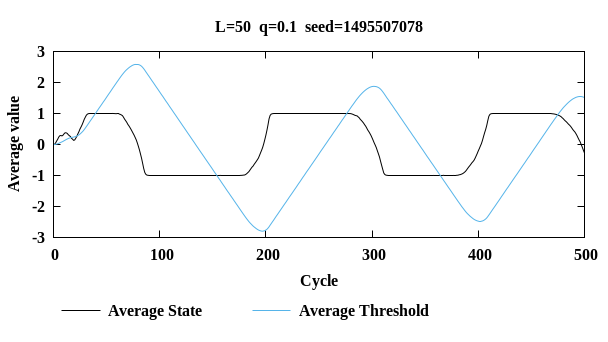
\includegraphics[width=.7\linewidth]{ICA-L50-q0_100-seed1495507078-AvgStateAvgThresVsCycle.png}
    \caption{É observado um comportamento de circuito RC espelhado horizontalmente.}
  \end{figure}

  \begin{figure}[h]
    \centering
    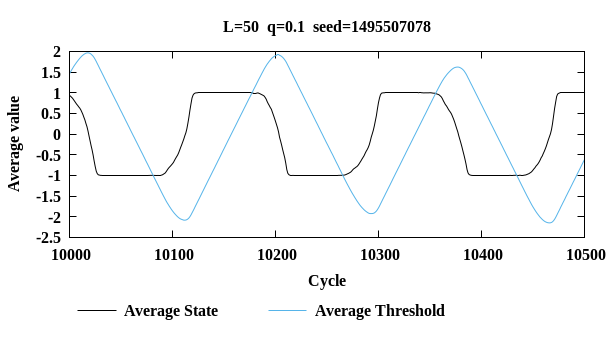
\includegraphics[width=.7\linewidth]{ICA-L50-q0_100-seed1495507078-AvgStateAvgThresVsCycle10000.png}
    \caption{O comportamento de circuito RC se mantém mesmo após vários ciclos.}
  \end{figure}

  \begin{figure}[h]
    \centering
    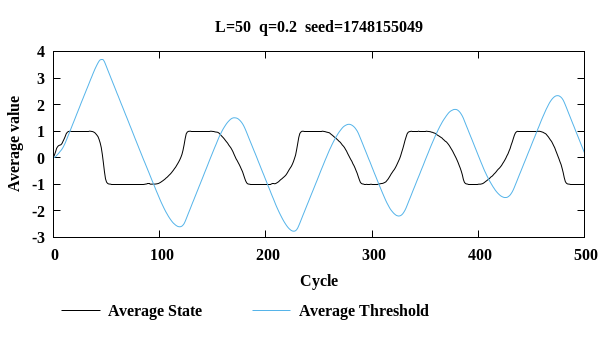
\includegraphics[width=.7\linewidth]{ICA-L50-q0_200-seed1748155049-AvgStateAvgThresVsCycle.png}
    \caption{}
  \end{figure}
  
  \begin{figure}[h]
    \centering
    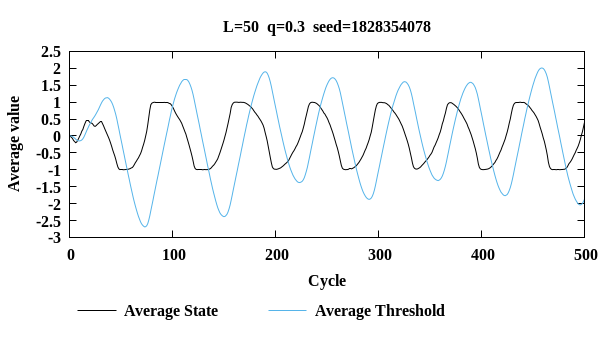
\includegraphics[width=.7\linewidth]{ICA-L50-q0_300-seed1828354078-AvgStateAvgThresVsCycle.png}
    \caption{}
  \end{figure}

  \begin{figure}[h]
    \centering
    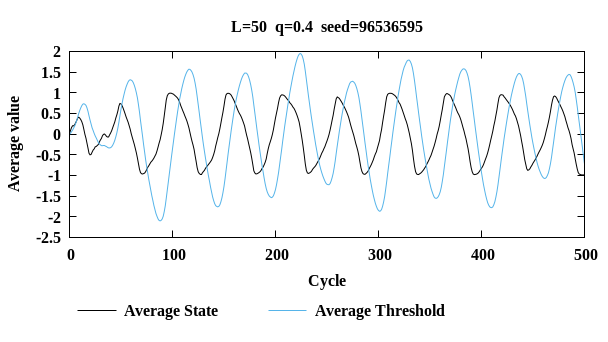
\includegraphics[width=.7\linewidth]{ICA-L50-q0_400-seed96536595-AvgStateAvgThresVsCycle.png}
    \caption{}
  \end{figure}
  
  \begin{figure}[h]
    \centering
    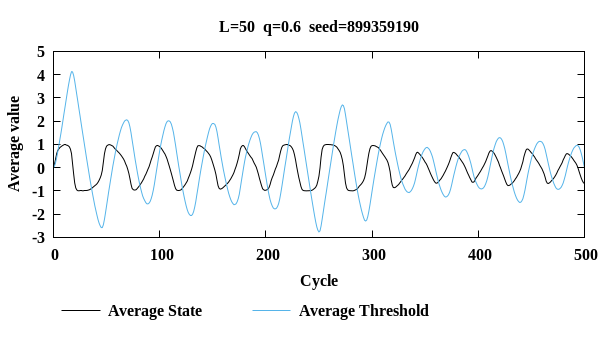
\includegraphics[width=.7\linewidth]{ICA-L50-q0_600-seed899359190-AvgStateAvgThresVsCycle.png}
    \caption{O comportamento de circuito RC aparece após o periodo de ``acomodamento''.}
  \end{figure}

  \begin{figure}[h]
    \centering
    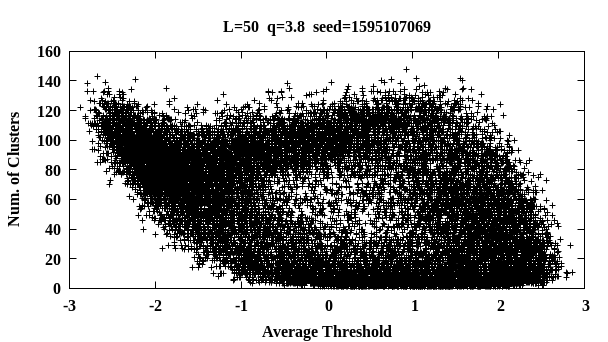
\includegraphics[width=.7\linewidth]{ICA-L50-q3_799-seed1595107069-ClusterVsAvgThres.png}
    \caption{Demonstração do comportamento caótico quando considerada uma vizinhança de Moore. O visual é igual ao observado para a vizinhança de Von Neumann.}
  \end{figure}

  \begin{figure}[h]
    \centering
    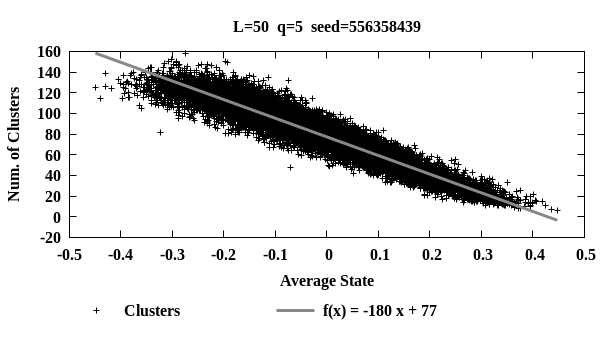
\includegraphics[width=.7\linewidth]{ICA-L50-q5_0-seed556358439-ClusterVsAvgState.png}
    \caption{Demonstração da relação linear entre número de aglomerados e estado médio quando a vizinhança é de Moore.}
  \end{figure}

  Foi pesquisada a definição de volatilidade: ``Volatilidade, na área financeira, é uma medida de dispersão dos retornos de um título ou índice de mercado. Quanto mais o preço de uma ação varia num período curto de tempo, maior o risco de se ganhar ou perder dinheiro negociando esta ação, e, por isso, a volatilidade é uma medida de risco.'' A volatilidade pode ser dada, entre outras maneiras, pelo desvio padrão no preço de um produto ou em um mercado. Considerando essa definição, é possível relacionar o preço com o limiar, e $q$ com a volatilidade.

  Para os próximos dias, estas serão as tarefas realizadas:
  \begin{enumerate}
    \item Escrita de um programa que utiliza o método dos mínimos quadrados para a obtenção da afinidade para os dados obtidos.
    \item Explicação do porquê de o limiar intrínseco a cada célula ser considerado como um determinador do momento certo para vender ou comprar;
    \item Simulação para as combinações com $L = 1000$ e $q\in\{$ 
    $0.2,$ $0.4,$ $0.6,$ $0.8,$ $1,$ 
    $1.2,$ $1.4,$ $1.6,$ $1.8,$ $2,$ 
    $2.2,$ $2.4,$ $2.6,$ $2.8,$ $3,$
    $3.2,$ $3.4,$ $3.6,$ $3.8,$ $4,$
    $4.2,$ $4.4,$ $4.6,$ $4.8,$ $5,$
    $5.2,$ $5.4,$ $5.6,$ $5.8,$ $6,$
    $6.2,$ $6.4,$ $6.6,$ $6.8,$ $7,$ 
    $7.2,$ $7.4,$ $7.6,$ $7.8,$ $8,$
    $8.2,$ $8.4,$ $8.6,$ $8.8,$ $9,$ 
    $9.2,$ $9.4,$ $9.6,$ $9.8,$ $10\}$, pois é nessa região que estão os dados que caracterizam a sigmóide;
	\end{enumerate}

\end{document}
